\documentclass[a4paper,12pt]{article}
\usepackage[utf8]{inputenc}
\usepackage{graphicx}
\usepackage{float}
\begin{document}
\begin{titlepage}
    \begin{center}
        \vspace*{1cm}
            
        \LARGE
        Project Title
            
        \vspace{0.5cm}
        \Huge
        \textbf{Human Action Recognition}
            
        \vspace{0.5cm}
            
        \textbf{Author \\}
            Naimul Hasan \\
            Md. Sabbir Irfan Chowdhury
            
        \vspace{6cm}
        \large
        \textbf{Report Written By:}\\
        Naimul Hasan \\
        Reg: 2017331059 \\
        Computer Science \& Engineering. \\
        Shahjalal University Of Science \& Technology \\
        \date{\today}
            
    \end{center}
\end{titlepage}
\thispagestyle{empty}
\section*{Abstract} 
Vision-based human action recognition has received increasing attentions in computer vision and has made significant progress in recent years. In vision-based action recognition tasks, a variety of human actions are inferred based on the complete movements of this action. Recurrent neural network (RNN) and long short-term memory (LSTM) have achieved great success in processing sequential multimedia data and yielded the state-of-the-art results in speech recognition, digital signal processing, video processing, and text data analysis. In this project, we use a convolutional neural network (CNN) for extracting features the video. First, deep features are extracted from the frame of the videos. Next, the sequential information among frame features is learnt using the LSTM network. The created model is capable of learning long term sequences and can process lengthy videos and detect action of the given input video. Our implemented model gave about 74-75\% validation accuracy on UCF101 dataset. Though it is not a good accuracy compares to the state-of-the art accuracy, yet it is not that bad even because we were limited by the resources and lack of knowledge of some other better techniques.
\newpage
\pagenumbering{roman}
\tableofcontents
\newpage
\pagenumbering{arabic}
\section{Introduction} Human action is the movement of parts of the body via interaction with objects in the environment. Video is a sequential data in which movements in visual contents are represented in many frames such that sequence of frames help in understanding the context of an action.\\ Action recognition in the video is the task of detecting the action in the video by analyzing the frames of the video. Action recognition in video sequences is a challenging problem of computer vision due to the similarity of visual contents\cite{nanda2019illumination}, changes in the viewpoint for the same actions, camera motion with action performer, scale and pose of an actor, and different illumination conditions \cite{soomro2012ucf101}. Human actions range from simple activity through arm or leg to complex integrated activity of combined arms, legs, and body.\\ One of the key motivations of action recognition is the vast domain of its applications in surveillance videos\cite{nanda2017neuromorphic}, robotics, human-computer interaction\cite{aly2013data}, sports analysis, video games for player characters, and management of web videos \cite{yue2015beyond}.Action recognition using video analysis is computationally expensive as processing a short video may take a long time due to its high frame rate. As each frame plays an important role in a video story, keeping information of sequential frames for long time, makes the system more efficient. In this project, we recognize human actions in a way similar to our observation of actions in real life. We use LSTM to consider the information of previous frames in automatic understanding of actions in videos. A kind of  Recurrent neural network called LSTM is used to analyze frame to frame change of action videos. RNNs are building blocks of a connected neuron with input units, internal (or hidden) units, and output units, having an activation at time t, which can selectively process data in sequence. As it processes one element at a time, it can model outputs, consisting of sequence of elements that are not independent\cite{lipton2015critical}. The RNN architecture provides strength to processing and finding hidden patterns in time-space data such as audio, video, and text. RNN processes data in sequential way such that at each time t, it gets input from the previous hidden state St−1 and new data xt. The data is also multiplied with weights, biases are added, and is fed to activation functions. Due to the large number of calculations, the effect of the initial inputs becomes negligible for the upcoming sequence of data after few layers, resulting in vanishing gradient problem. The solution to this problem is LSTM. The main idea of LSTM architecture is its memory cell, input gate, output gate, and forget gate, which can maintain its state over time TN, and non-linear gating units which regulate the information flow into/out of the cell\cite{greff2016lstm}. \\
\section{Related works}
Over the last decade, researchers have presented many hand-crafted and deep-nets based approaches for action recognition. The earlier work was based on hand-crafted features for non-realistic actions, where an actor used to perform some actions in a scene with simple background. Such systems extract low level features from the video data and then feed them to a classifier such as support vector machine (SVM), decision tree, and KNN for action recognition.These methods were not feasible for complex and lengthy video. To process complex datasets, we need hybrid approaches which can combine different features and preprocessing such as motion detection \cite{choudhury2016evaluation}, background segmentation \cite{choudhury2017segmenting}, HOG, SIFT, and SURF. But such hybrid methods increase the computational complexity of the target system. These limitations can cause difficulty for lengthy videos and real-time applications with continuous video streaming. Besides hand-crafted features based approaches for action recognition, several deep learning based methods were also proposed in recent years. Deep learning has shown significant improvement in many areas such as image classification, person re-identification, object detection, speech recognition and bioinformatics \cite{choudhury2018improved}. For instance, a straight forward implementation of action recognition using deep networks is developed through 3D convolutional networks by Ji et al. \cite{ji20123d}. They applied 3D convolutional kernels on video frames in a time axis to capture both spatial and temporal information. They also claimed that their approach can capture motion and optical flow information because frames are connected by fully connected layers at the end. A multi-resolution CNN framework for connectivity of features in time domain is proposed by \cite{karpathy2014large} to capture local spatio-temporal information. This method is experimentally evaluated on a new YouTube 1 million videos dataset of 487 classes. The authors claimed to have speed up the training complexity by foveated architecture of CNN. They improved the recognition rate for large dataset up to 63.9\% but their recognition rate on UCF101 is 63.3\%, which is still too low for such important task of action recognition. A two-stream CNN architecture is proposed by \cite{simonyan2014two} in which first stream captures spatial and temporal information between frames and second one demonstrates the dense optical flow of multiple frames. They have increased the amount of data for the training CNN model by combining two datasets. Deep learning based approaches have the ability to accurately identify hidden patterns in visual data because of its huge feature representation pipeline. On the other hand, it requires huge amount of data for training and high computational power for its processing. In this work, we have balanced the complexity of the system and action recognition accuracy. For better action recognition, we have intelligently combined CNN and LSTM due to its state-of-the-art results on visual and sequential data.

\section{Methodology}
We used “Google Colab” to run the programs. It provides us approx. 12 GB of RAM and variable GPU depending on the traffic.
Steps include:
\begin{enumerate}
    \item Working with the dataset.
    \item Extracting features from the frames using CNN.
    \item Passing those features into a recurrent neural network to train the model and classifying the videos based on that.
    \item Saving the best model and then using it to classify the videos.
\end{enumerate}
\subsection{Dataset}
UCF101 is one of the most popular action recognition datasets of realistic action videos. It consists of 13320 videos taken from YouTube, which are divided into 101 action categories. Each category contains videos between [100, 200]. UCF101 is comparatively more challenging dataset due to its large number of action categories from five major types: 1) human-object interaction, 2) body-motion only, 3) humanhuman interaction, 4) playing musical instruments, and 5) sports. Some categories have many actions such as sports, where most of the sports are played in a similar background, i.e., greenery. Some of the videos are captured in different illuminations, poses, and from different viewpoints. One of the major challenges in this dataset is its realistic actions performed in real life, which is unique compared to other datasets where actions are performed by an actor. 
\subsection{Working with the dataset}
We downloaded the dataset “UCF101” and extracted in google drive. It contains 13320 videos belonging to 101 different classes. Then we separated the video in two folders namely “test” and “train”. This splitting was based on the test train spilt file provided in their official site. Then, we extracted the frames from each video in their corresponding folders as .jpg files
\subsection{Preparation and features extraction}
To extract features from the images, we used a pre-trained model provided by Keras named Inception-V3. Inception-V3 is a model provided by Keras whose weights pre-trained on ImageNet dataset, which is a huge dataset consisting of large number of images of different classes. It saves us from building our own architecture from scratch which could take far more time and efforts and not necessarily provide better results than when using Inception-V3. Thus, in our project we used this Inception-V3 model to extract features. In our initial work, we just settled with this work by fine tuning some outermost layers and predicting the class solely based on this. But, we improved our design by using RNN which is shown in next step.
\subsection{Passing the features to RNN and training the model}
Instead of classifying the images just with CNN, we now use CNN+RNN model. Here the feature output from Inception-V3 are first taken by removing the top classifying layer. It gives a vector of features. We used LSTM, which is a special kind of RNN. It is also provided by keras in python. The features we obtained from Inception-V3, are passed to this LSTM architecture. After that, we defined some of our own layers. We tried with dense layers with ‘relu’ activation with some dropouts between multiple layers. After trying with different layers, we settled down to a 2048-wide LSTM layer followed by a 512 dense layer and used 0.5 dropout. Note that we used the features from a video as input to the LSTM. Instead of passing features from every frame, we reduced the number of frames to be passed. This reduced overfitting and also made the program faster due to less features being processed now. Features from approx. 30-50 frames per video are sent as sequence to the LSTM. At the final layer, we used ‘softmax’ activation, which is basically used to provide a class as output in terms of probability, i.e. it turns the input numbers to probabilities that sum to 1. Thus, it outputs a probability distribution. We used “categorical cross entropy” as a loss measure and adam optimizer was used with learning rate of .Also, the metrics for training and testing was ‘accuracy’ and ‘top 5 categorical accuracy’. Then we compiled our model using these parameters and are ready for training. \\Thus training is based on above mentioned architecture. The training and testing samples are divided according to the file provided in official website. This ensures uniform division of videos. The model is trained to learn in such a way to minimize the validation loss. When we stop learning, i.e. the validation loss keeps on increasing, then we stop the training. The accuracy metrics is used. When doing the training, we save the model weights whenever validation loss is decreased. When training finishes, we get the recently saved weights as the best weights and we will use those weights further in classifying our own videos. 
\subsection{ Saving the best model and classifying Videos}
As written above, we have saved the model weights for that iteration where we get the least validation loss. This is generally a good practice because if we save model with best accuracy only, no matter what the loss is, then we can’t say that it is the best model. So, least loss is what we used when specifying the best model. Although it may vary depending on the tasks given, but generally for HAR, it is good enough. Now, to classify videos, we just define the same architecture we defined for training. Then we load the model weights and now we are ready to classify the videos. Just take a video, extract frames and then use Inception-V3 to extract features from that video. Pass those features into the architecture and we get the class to which the video belongs.
\section{Experimental evaluation}
We trained our model on UCF101 dataset using the architecture described in the previous section and the results were obtained. We experimented with different hidden layers added to our architecture so as to get the best model. Earlier the method we used included CNN only and the validation accuracy was very low in that case when compared to the new model we defined. The following graphs shows various accuracies and loss we found out during the experiment:
\begin{figure}[H]
    \centering
    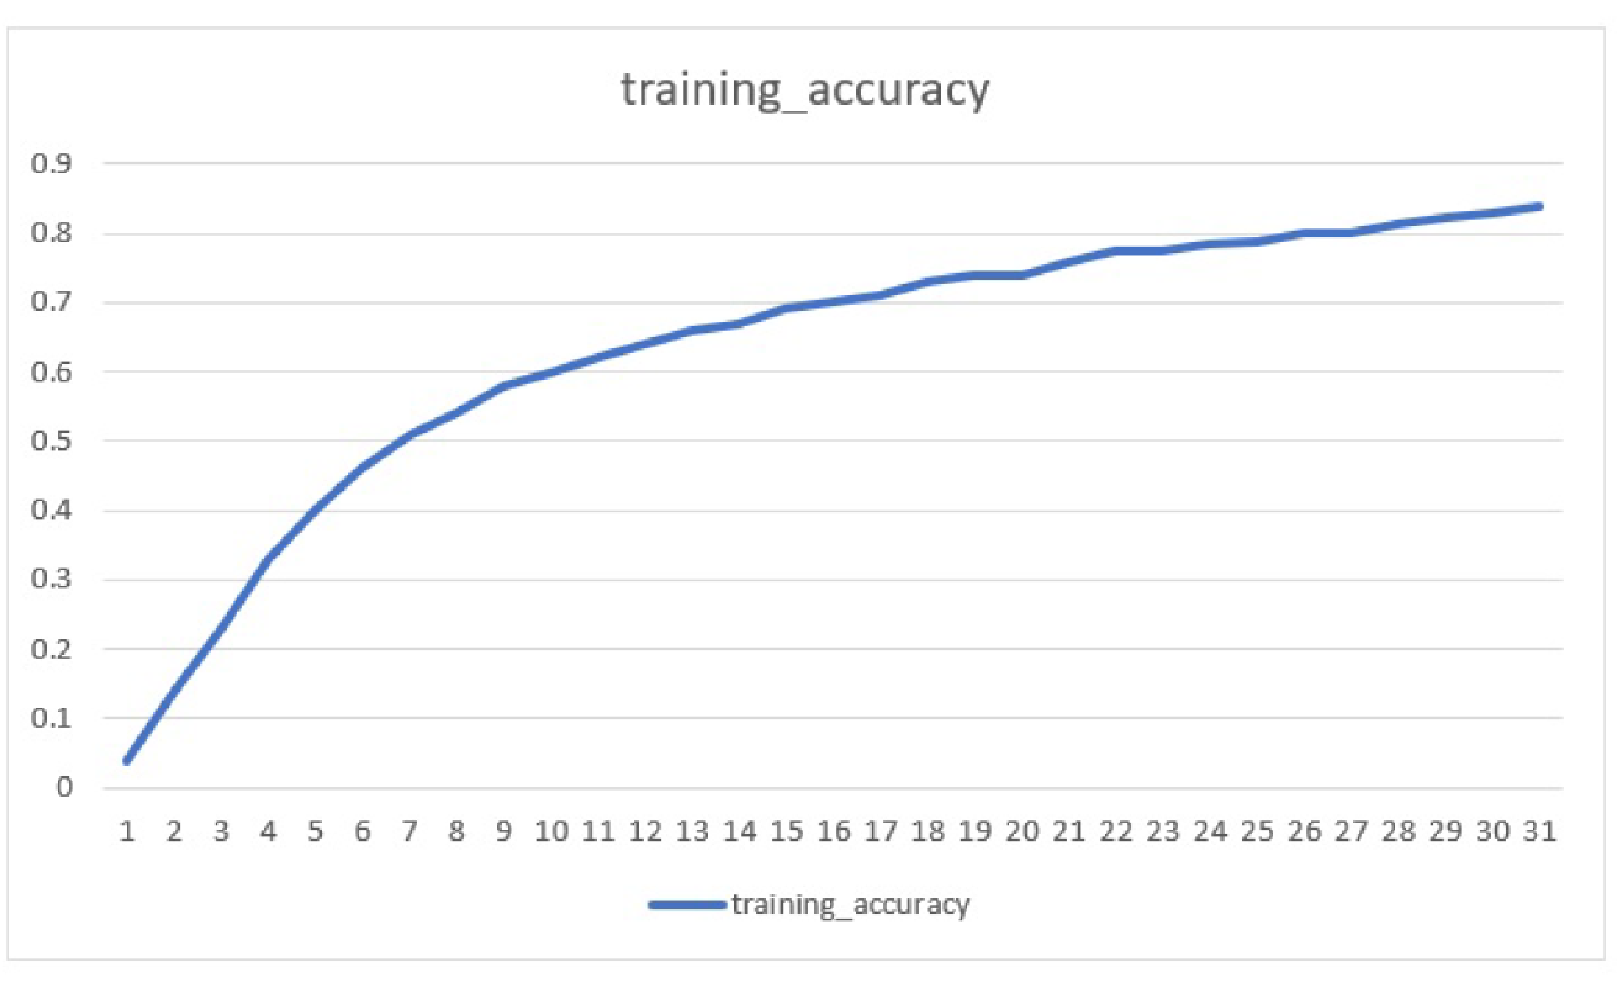
\includegraphics[width=1\textwidth]{training_aacuracy}
    \caption{Training accuracy}
    \label{fig:my_label}
\end{figure}
We reached training accuracy of approx. 84 percent and that accuracy was achieved at around 30 epochs.
\begin{figure}[H]
    \centering
    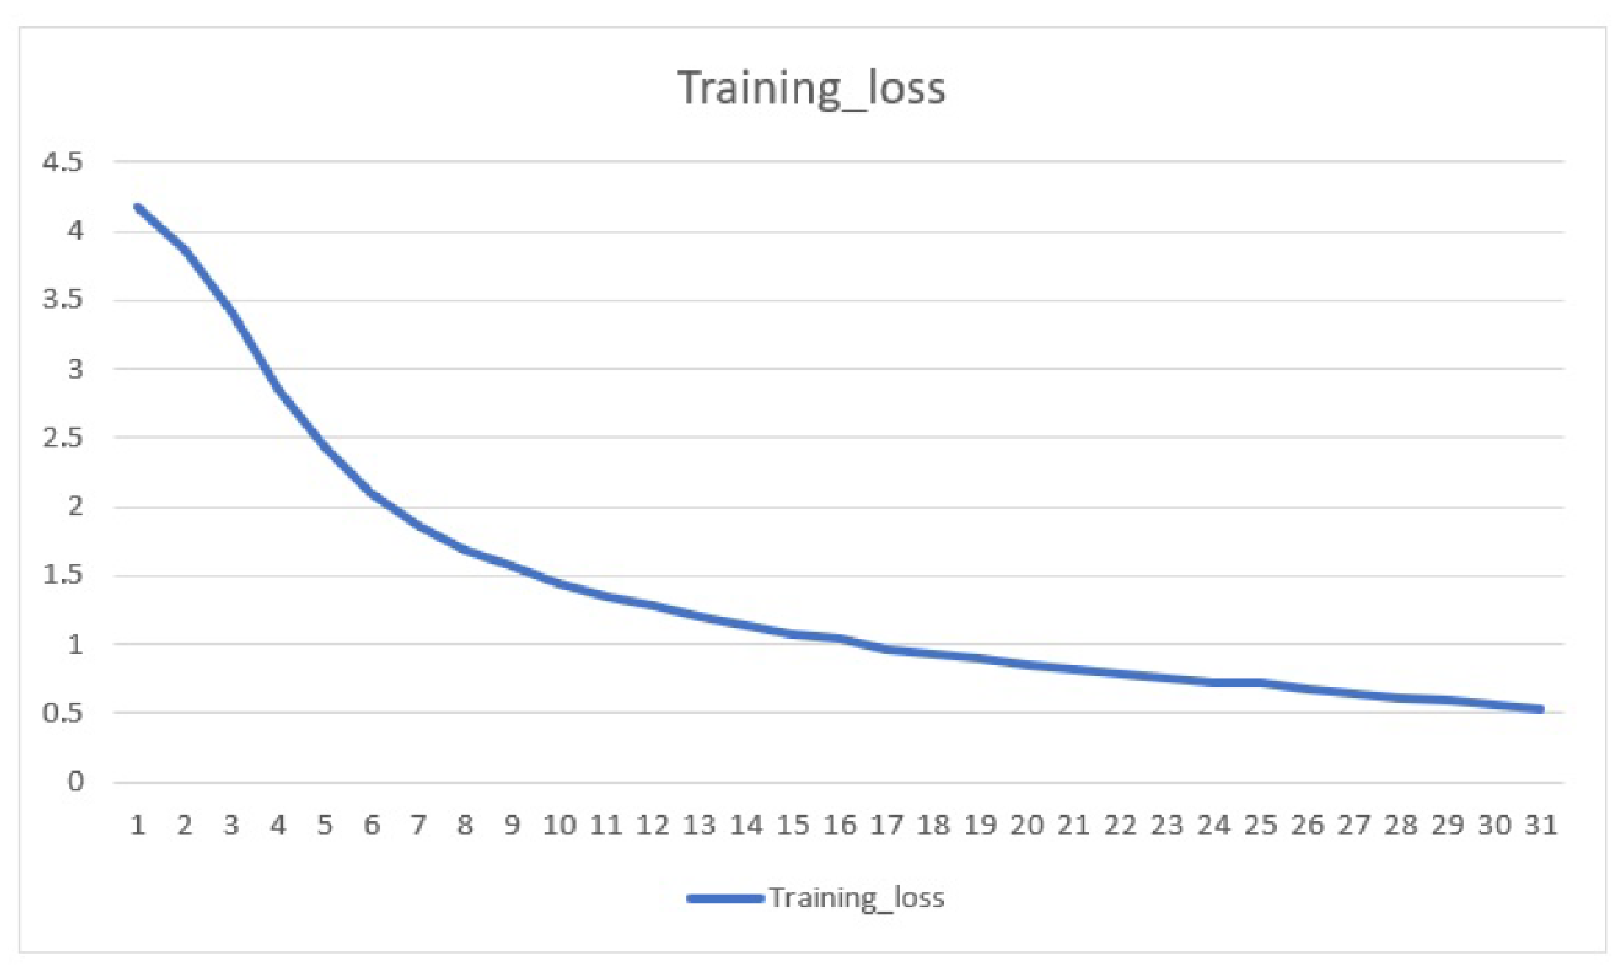
\includegraphics[width=1\textwidth]{training_loss}
    \caption{Training loss}
    \label{fig:my_label}
\end{figure}
The training loss decreased with number of epochs. It dropped down from 4.2 to 0.6 with 30 epochs.
\begin{figure}[H]
    \centering
    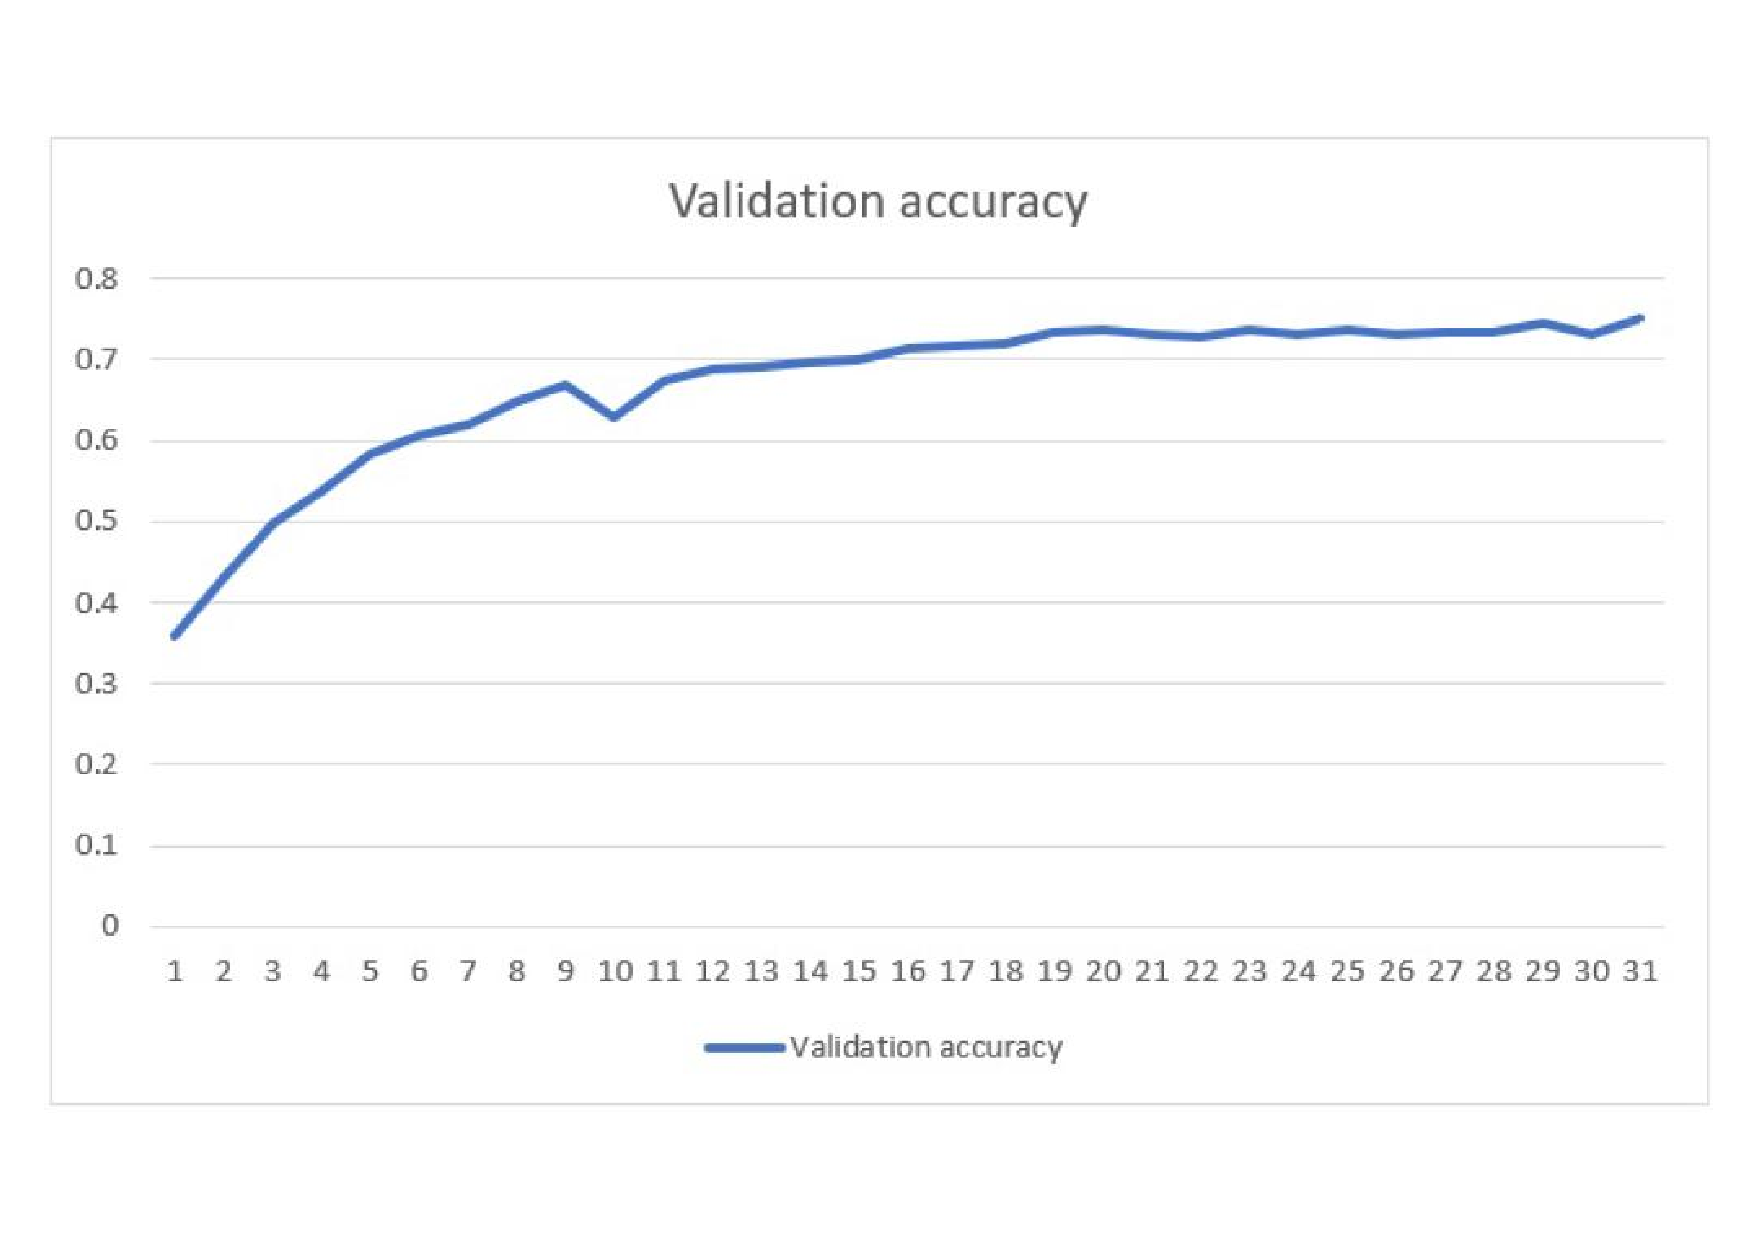
\includegraphics[width=1\textwidth]{validation_accuracy_init-converted}
    \caption{validation accuracy}
    \label{fig:my_label}
\end{figure}
The validation accuracy we got on UCF101 data was around 74 percent and was achieved with 30 epochs. The validation loss was initially 3.8 and gradually it decreases to around 1 after 30 epochs. In CNN only model, we obtained best loss of 7.2 which is much higher than what we obtained in our new model which was nearly 1.
We reached around 25 percent accuracy only on validation data when using the CNN model only. This is very much less compared to 74 percent accuracy we obtained on CNN+RNN model.
\section{Conclusion}
The implemented model gave about 74-75\% validation accuracy on such a big dataset UCF101. And the loss was approximately 1. Whereas, the previous model just gave 25\% accuracy with a higher loss. Although this 74\% accuracy achieved is not that good when compared to 94\% state-of-the art accuracy, yet it is not that bad even because we were limited by the resources and lack of knowledge of some other better techniques.
During this whole project, we learned many new things.
We learned about neural network, their different types: CNN and RNN. Since we had to study them in detail for the implementation, it enhanced our knowledge about neural networks. With these learnings, we hope to work more towards this field as in the future most of the things will be computational and we would like to keep pace with it. Also, it is very interesting to learn that how a machine is made to act and think like humans. We learned about Human Action Recognition methods and also how it can very useful in several applications. We learned many new libraries provided in Python. It makes it easy to implement our ideas. Main focus of learning was CNN and RNN. We learnt them from scratch and also saw various applications where these can be used.
\newpage
\bibliographystyle{ieeetr}
\bibliography{references} 
\end{document}
